% =====================================================================
%  SchemaLens-Cassandra (RUBiS V9) -- Versao ajustada v1
%  E20 refeito neste servidor: dados regenerados, Cassandra 4.1.12 e 3.11.11.
%  Tabelas em tables/ (rubis_v1/make_tables.py); figuras em figs/.
% =====================================================================
\documentclass[11pt,a4paper]{article}
\usepackage[T1]{fontenc}
\usepackage[utf8]{inputenc}
\usepackage{lmodern}
\IfFileExists{brazil.ldf}{\usepackage[brazil]{babel}}{}
\usepackage[a4paper,margin=2.0cm]{geometry}
\usepackage{amsmath,amssymb,graphicx,booktabs,tabularx,longtable,array,float}
\usepackage[font=small,labelfont=bf]{caption}
\usepackage[table]{xcolor}
\usepackage{microtype,fancyhdr}
\usepackage[colorlinks=true,linkcolor=blue!50!black,urlcolor=blue!50!black]{hyperref}
\definecolor{boxbg}{RGB}{243,246,250}
\definecolor{warnbg}{RGB}{253,244,232}
\newcommand{\caixa}[2][boxbg]{\par\smallskip\noindent\colorbox{#1}{\parbox{\dimexpr\linewidth-2\fboxsep}{#2}}\par\smallskip}
\newcommand{\just}[1]{\caixa{\textbf{Justificativa.} #1}}
\newcommand{\limit}[1]{\caixa[warnbg]{\textbf{Limitação.} #1}}
\newcolumntype{Y}{>{\raggedright\arraybackslash}X}
\newcommand{\envstarted}{2026-11-17 21:52}
\newcommand{\envfinished}{2026-11-18 00:37}
\newcommand{\envpython}{3.12.3}
\newcommand{\envdriver}{3.30.1}
\newcommand{\envcpuset}{0-3}
\newcommand{\envrawrows}{3.600.000}
\newcommand{\envdiscarded}{0}
\newcommand{\envhtopA}{H01, H02}
\newcommand{\envhtopB}{H01, H02, H03, H04, H05}
\newcommand{\envoracleN}{397.479}

\makeatletter\newcommand{\tabin}[1]{\@@input #1 }\makeatother
\newcommand{\optinput}[1]{\IfFileExists{#1}{\input{#1}}{\emph{[texto a escrever após a análise]}}}
\pagestyle{fancy}\fancyhf{}
\lhead{\small SchemaLens--Cassandra (RUBiS V9) --- versão ajustada v1}\rhead{\small Relatório de execução}\cfoot{\thepage}

\title{\textbf{SchemaLens--Cassandra com o RUBiS (V9)}\\[4pt]\large Versão ajustada: E20 refeito sob o protocolo comum v1,\\ com dados regenerados e Cassandra 4.1.12 $\times$ 3.11.11}
\author{Projeto SchemaLens / Cassandra}
\date{Execução: \envstarted--\envfinished{} UTC}

\begin{document}
\maketitle
\begin{abstract}
\noindent A análise de consistência apontou que o RUBiS V9 foi medido em Cassandra 3.11.11, enquanto os três benchmarks TSDB usaram 4.1.x (crítico 2), e que a estatística era diferente (crítico 3). O \texttt{rubis\_full} da V9 existe só na máquina original e foi gerado sem semente. Por isso esta versão refaz o E20 neste servidor, em quatro passos:
\begin{itemize}
\item \textbf{regenera} a fonte da coorte, reconstruindo a estrutura a partir das estatísticas do E04 e das convenções do código da V8, com valores no contrato do \texttt{fake.js};
\item \textbf{congela} H01--H05 da V9 sem alteração;
\item \textbf{mede} os 9 deployments (H01--H05, NoSE, QPG, V8\_AUTO\_H\_norm e uma réplica A/A) com os \textbf{mesmos dados em dois nós dedicados, 4.1.12 e 3.11.11}, intercalados em ABBA;
\item \textbf{confere} cada resposta contra o oráculo independente da V9 (\envoracleN{} respostas esperadas por deployment e versão).
\end{itemize}
Foram \envrawrows{} requisições medidas. \optinput{tables/abstract_result.tex}
\end{abstract}
\tableofcontents\newpage

\section{Resumo executivo}
\optinput{tables/exec_summary.tex}

\section{Por que regenerar os dados e como}
\paragraph{Restrição.} O \texttt{rubis\_full} (70,4 M linhas), o repositório da V8 (hashes de referência) e as latências brutas da V9 estão só na máquina original. O gerador da V8 não foi preservado; o \texttt{InitDBSQL} Java de \texttt{rubis2/} é outro gerador.

\paragraph{Reconstrução} (\texttt{rubis\_v1/gen\_data.py}, semente 20261117):
\begin{itemize}
\item \textbf{Estrutura}: modular, reconstruída dos fan-outs exatos do E04 (10 itens por vendedor, 4.000 itens por categoria, 4.000 usuários por região, 500 pares região $\times$ categoria, 10 lances por item, 100 por usuário etc.) e das convenções do código do fecho da V8 (\texttt{uid + k$\cdot$200000}).
\item \textbf{Valores}: contrato do \texttt{fake.js} do NoSE, com um gerador pseudoaleatório por linha.
\item \textbf{Datas monótonas no id}: o NoSE, cujas tabelas ordenam por id, concordava 100\% com o contrato (que ordena por data) na V9. A primeira tentativa, com datas sorteadas, falhou no smoke nesse ponto e está arquivada em \texttt{attempts/}.
\item \textbf{Coorte}: as 5 primeiras páginas de 1.000 linhas na ordem de token Murmur3 (\texttt{baselines\_005.materialize}) $\cup$ o fecho do domínio, pela regra de \texttt{benchmark\_005}.
\end{itemize}
\begin{table}[H]\centering\small\caption{Coorte reconstruída $\times$ coorte da V9.}
\begin{tabular}{@{}lrr@{}}\toprule Entidade & Reconstruída & V9\\\midrule\tabin{tables/t_cohort.tex}\bottomrule\end{tabular}\end{table}
\just{Lances e buynow coincidem exatamente com a V9 (5.690 e 5.300), e comentários quase (6.529 contra 6.501), o que confirma a regra da coorte. Usuários e itens ficam maiores, porque a V8 acrescentava menos pais numa etapa de enriquecimento cuja regra não foi preservada. O estado lido pela V9 tem escala próxima (21.855 usuários contra 20.494).}
\limit{Estes \emph{não} são os dados da V9. A comparação de valores absolutos com a V9 mistura duas mudanças (dados e versão). Por isso a comparação de versão é feita \emph{aqui}, com os mesmos dados nas duas versões.}

\section{Protocolo}
\begin{table}[H]\centering\small
\begin{tabularx}{\linewidth}{@{}lY@{}}\toprule
Nós & \texttt{sl\_v1\_rubis\_cassandra} (4.1.12, imagem do protocolo v1, porta 9064) e \texttt{sl\_v1\_rubis311\_cassandra} (3.11.11, \texttt{sha256:5e13c93d\ldots}, porta 9065); CPUs \envcpuset, 6\,GB, heap 2\,GB; só um nó ligado por vez\\
Dados & mesma coorte nos dois nós; hashes de \texttt{load\_raw\_state} e \texttt{source\_closure} (funções da V9) idênticos; keyspaces materializados idênticos\\
Requisições & protocolo da V9 sem alteração: 4 cargas, 1.000 aquecimentos + 10.000 medidas, histórias semeadas, \texttt{reset\_state} antes e depois\\
Repetições & 5; antes de cada (repetição, versão): flush, reinício a frio, gate; versões em ABBA; deployments na ordem da V9 (ímpar) ou invertida (par)\\
Corretude & oráculo independente da V9 (\texttt{oracle\_v9.py}, contrato E6) com o mesmo histórico de escritas\\
Isolamento & \texttt{BulkWriterWatch} da V9 + \texttt{compaction\_history} (simétrico nas duas versões)\\
Cliente & Python \envpython, driver \envdriver; janelas descartadas: \envdiscarded\\\bottomrule
\end{tabularx}\end{table}
\limit{No braço 4.1.12, o DDL congelado do V8\_AUTO\_H\_norm, capturado do 3.11, trazia \texttt{dclocal\_read\_repair\_chance} e \texttt{read\_repair\_chance}, que foram removidas no 4.0. Elas foram retiradas em memória; os valores eram os padrões do 3.11 e, com RF\,=\,1, sem efeito. O E23 (escala completa) não foi refeito.}

\section{Resultados}
\subsection{Latência média por carga}
{\small\begin{longtable}{@{}lcccc@{}}
\caption{Cassandra 4.1.12: média por requisição (ms) e IC 95\% bootstrap pareado.}\\
\toprule Deployment & Browsing & Bidding & Update10x & Update100x\\\midrule\endhead
\tabin{tables/t_mean_v41.tex}
\bottomrule\end{longtable}}
{\small\begin{longtable}{@{}lcccc@{}}
\caption{Cassandra 3.11.11: média por requisição (ms) e IC 95\% bootstrap pareado.}\\
\toprule Deployment & Browsing & Bidding & Update10x & Update100x\\\midrule\endhead
\tabin{tables/t_mean_v311.tex}
\bottomrule\end{longtable}}
\begin{figure}[H]\centering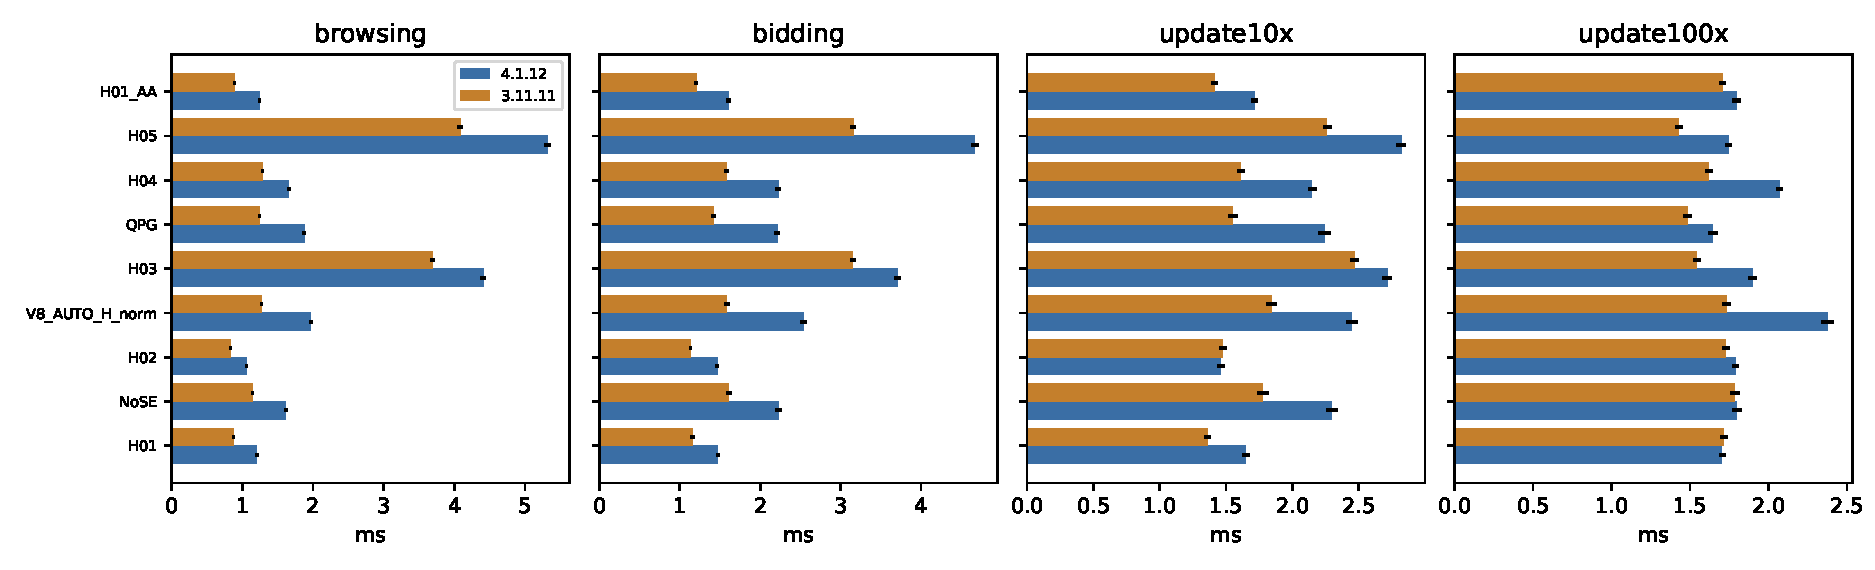
\includegraphics[width=\linewidth]{figs/fig_v1_rubis.pdf}\caption{Média por carga nas duas versões (mesmos dados, mesmo protocolo).}\end{figure}
\optinput{tables/mean_text.tex}

\subsection{Contrastes com os baselines}
{\scriptsize\setlength{\tabcolsep}{2.5pt}\begin{longtable}{@{}llcccc@{}}
\caption{Razão H/baseline em 4.1.12 / 3.11.11. \textbf{H+}: H mais rápido; H$-$: mais lento; empate: IC pareado contém 1 ou diferença abaixo do piso de ruído.}\\
\toprule H & Baseline & Browsing & Bidding & Update10x & Update100x\\\midrule\endhead
\tabin{tables/t_contrasts.tex}
\bottomrule\end{longtable}}

\subsection{Previsto $\times$ medido dentro de H}
{\scriptsize\setlength{\tabcolsep}{3pt}\begin{longtable}{@{}llllcccc@{}}
\toprule Versão & Carga & Ordem prevista & Ordem medida & $\tau$ & Top-1 & Regret & Piso\\\midrule\endhead
\tabin{tables/t_withinH.tex}
\bottomrule\end{longtable}}
Htop (não dominados nas 4 cargas): 4.1.12 = \envhtopA; 3.11.11 = \envhtopB.

\subsection{Efeito da versão (mesmos dados)}
{\small\begin{longtable}{@{}lcccc@{}}
\caption{Razão das médias 4.1.12 / 3.11.11 (menor que 1: 4.1 mais rápido) e $\tau$ de Kendall entre as ordenações.}\\
\toprule Deployment & Browsing & Bidding & Update10x & Update100x\\\midrule\endhead
\tabin{tables/t_versions.tex}
\bottomrule\end{longtable}}
\optinput{tables/versions_text.tex}

{\small\begin{longtable}{@{}lcccc@{}}
\caption{4.1.12: p50 / p95 / p99 (ms).}\\
\toprule Deployment & Browsing & Bidding & Update10x & Update100x\\\midrule\endhead
\tabin{tables/t_pct_v41.tex}
\bottomrule\end{longtable}}

\section{Hipóteses pré-registradas}
\begin{longtable}{@{}p{0.7cm}p{6cm}p{1.8cm}p{6.6cm}@{}}
\toprule & Hipótese & Resultado & Evidência\\\midrule\endhead
\tabin{tables/t_hyp.tex}
\bottomrule\end{longtable}

\section{Aceitação}
\begin{minipage}[t]{0.52\linewidth}\small\begin{tabular}[t]{@{}lc@{}}\toprule Gate & \\\midrule\tabin{tables/t_gates.tex}\bottomrule\end{tabular}\end{minipage}\hfill
\begin{minipage}[t]{0.46\linewidth}\small\begin{tabular}[t]{@{}lc@{}}\toprule Teste negativo & \\\midrule\tabin{tables/t_neg.tex}\bottomrule\end{tabular}\end{minipage}

\section{Conclusões}
\optinput{tables/conclusions.tex}

\appendix
\section{Reprodução (neste servidor)}
\begin{verbatim}
cd versao_ajustada/rubis_v9
./run_server.sh gen | node | import | oracle | smoke | freeze
./run_server.sh measure | analyze | accept | report
\end{verbatim}
\end{document}
